\documentclass[main.tex,fontsize=8pt,paper=a4,paper=portrait,DIV=calc,]{scrartcl}
% Document
\usepackage[T1]{fontenc}
\usepackage[utf8]{inputenc}
\usepackage[dvipsnames]{xcolor}
\usepackage[nswissgerman,english]{babel} 
\usepackage{hyperref}
\renewcommand{\familydefault}{\sfdefault}

% Format
\usepackage[top=5mm,bottom=1mm,left=5mm,right=5mm]{geometry}
%\setlength{\headheight}{\baselineskip}
%\setlength{\headsep}{0mm}

%\usepackage{scrlayer-scrpage}
%\clearpairofpagestyles
%\chead{{\bfseries\TITLE, \AUTHOR, \pagename~\thepage}}

%\addtokomafont{pagehead}{\upshape}

\usepackage{multicol}
\setlength{\columnsep}{2mm}
\setlength{\columnseprule}{0.1pt}

% Math
\usepackage{amsmath}
\usepackage{amssymb}
\usepackage{amsfonts}

% Code
\usepackage{fancyvrb, etoolbox, listings, xcolor}
%\usemintedstyle{bw}

%\newminted[shell]{bash}{
%fontsize=\footnotesize,
%fontfamily=tt,
%breaklines=true,
%frame=single,
%framerule=0.1pt,
%framesep=2mm,
%tabsize=2
%}
%\newminted{css}{
%breaklines=true,
%tabsize=4,
%autogobble=true,
%escapeinside=||,
%stripall=true,
%stripnl=true,
%}

    \definecolor{lightgray}{rgb}{0.95, 0.95, 0.95}
    \definecolor{darkgray}{rgb}{0.4, 0.4, 0.4}
    \definecolor{purple}{rgb}{0.65, 0.12, 0.82}
    \definecolor{ocherCode}{rgb}{1, 0.5, 0} % #FF7F00 -> rgb(239, 169, 0)
    \definecolor{blueCode}{rgb}{0, 0, 0.93} % #0000EE -> rgb(0, 0, 238)
    \definecolor{greenCode}{rgb}{0, 0.6, 0} % #009900 -> rgb(0, 153, 0)
    \definecolor{teal}{rgb}{0.0, 0.5, 0.5}

\lstdefinestyle{code}{
    identifierstyle=\color{black},
    keywordstyle=\color{blue}\bfseries\small,
    ndkeywordstyle=\color{greenCode}\bfseries\small,
    stringstyle=\color{ocherCode}\ttfamily\small,
    commentstyle=\color{teal}\ttfamily\textit\small,
    basicstyle=\ttfamily\small,
    breakatwhitespace=false,         
    breaklines=true,                 
    captionpos=b,                    
    keepspaces=true,                 
    showspaces=false,                
    showstringspaces=false,
    showtabs=false,                  
    tabsize=2,
    belowskip=-5pt
}



% Images
\usepackage{graphicx}
\newcommand{\pic}{\includegraphics[scale=0.3]}
\graphicspath{{Screenshots/}{../Screenshots}}
\makeatletter
\def\pictext#1#2{%
    \@ifnextchar[{%
    \pictext@iiiii{#1}{#2}%
    }{%
      \pictext@iiiii{#1}{#2}[0.5,0.4,0.3]% Default is 5
    }%
}
\def\pictext@iiiii#1#2[#3,#4,#5]{\begin{minipage}{#3\textwidth}\includegraphics[scale=#4]{#1}\end{minipage}\begin{minipage}{#5\textwidth}#2\end{minipage}}
\def\minipg#1#2{%
    \@ifnextchar[{%
    \minipg@iiii{#1}{#2}%
    }{%
      \minipg@iiii{#1}{#2}[0.3,0.6]% Default is 5
    }%
}
\def\minipg@iiii#1#2[#3,#4]{\vspace{0.8mm}\begin{minipage}{#3\textwidth}#1\end{minipage}\begin{minipage}{#4\textwidth}#2\end{minipage}{\vspace{0.8mm}}}
\makeatother

%\newenvironment{minty}[2]% environment name
%{% begin code
%  \begin{minipage}{#1}
%  \begin{minted}{#2}
%}%
%{% end code
%  \end{minted}
%  \end{minipage}
%  \end{minty}\ignorespacesafterend
%} 

% Smaller Lists
\usepackage{enumitem}
\setlist[itemize,enumerate]{leftmargin=3mm, labelindent=0mm, labelwidth=1mm, labelsep=1mm, nosep}
\setlist[description]{leftmargin=0mm, nosep}
\setlength{\parindent}{0cm}

% Smaller Titles
\usepackage[explicit]{titlesec}

%% Color Boxes
\newcommand{\sectioncolor}[1]{\colorbox{black!60}{\parbox{0.989\linewidth}{\color{white}#1}}}
\newcommand{\subsectioncolor}[1]{\colorbox{black!50}{\parbox{0.989\linewidth}{\color{white}#1}}}
\newcommand{\subsubsectioncolor}[1]{\colorbox{black!40}{\parbox{0.989\linewidth}{\color{white}#1}}}
\newcommand{\paragraphcolor}[1]{\colorbox{black!30}{\parbox{0.989\linewidth}{\color{white}#1}}}
\newcommand{\subparagraphcolor}[1]{\colorbox{black!20}{\parbox{0.989\linewidth}{\color{white}#1}}}

%% Title Format
\titleformat{\section}{\vspace{0.5mm}\bfseries}{}{0mm}{\sectioncolor{\thesection~#1}}[{\vspace{0.5mm}}]
\titleformat{\subsection}{\vspace{0.5mm}\bfseries}{}{0mm}{\subsectioncolor{\thesubsection~#1}}[{\vspace{0.5mm}}]
\titleformat{\subsubsection}{\vspace{0.5mm}\bfseries}{}{0mm}{\subsubsectioncolor{\thesubsubsection~#1}}[{\vspace{0.5mm}}]
\titleformat{\paragraph}{\vspace{0.5mm}\bfseries}{}{0mm}{\paragraphcolor{\theparagraph~#1}}[{\vspace{0.5mm}}]
\titleformat{\subparagraph}{\vspace{0.5mm}\bfseries}{}{0mm}{\subparagraphcolor{\thesubparagraph~#1}}[{\vspace{0.5mm}}]

%% Title Spacing
\titlespacing{\section}{0mm}{0mm}{0mm}
\titlespacing{\subsection}{0mm}{0mm}{0mm}
\titlespacing{\subsubsection}{0mm}{0mm}{0mm}
\titlespacing{\paragraph}{0mm}{0mm}{0mm}
\titlespacing{\subparagraph}{0mm}{0mm}{0mm}

%% format cells
\usepackage[document]{ragged2e}
\usepackage{array, makecell}
\renewcommand{\arraystretch}{2}
\newcommand{\mc}{\makecell[{{m{1\linewidth}}}]}



\begin{document}
\tableofcontents

\lstset{
    language=c++,
    style=code,
}

\newcommand{\TITLE}{CPP Advanced}
\newcommand{\AUTHOR}{Fabio Lenherr}
\setcounter{tocdepth}{1}

\section{Move Semantics}

\subsection{Copy}
\textcolor{purple}{By default cpp will always create copies, this is good for memory safety etc, as you will not be returning null values, but it can be a runtime hit!}\newline
\textcolor{teal}{(There are some special types that can't be copied like mutexes etc)}
\begin{lstlisting}
// Copy contructor
class something {
  something(const something &other) {
    // copy values from other
  }
}
\end{lstlisting}

\subsection{Move}
\textcolor{purple}{Move constructor will \emph{NOT copy values, instead, it will move these values into the new object, this is better for performance, but it requires more management from the programmer!}}\newline
\textcolor{teal}{Make sure to free the memory at the old object, otherwise you might be dealing with nullpointers!}
\begin{lstlisting}
Vector(Vector<T> &&vec)
    : size(vec.size), cap(vec.cap), data(std::move(vec.data)) {
  vec.data = nullptr;
} // yes this is the vector that you implemented kekw
\end{lstlisting}
\textcolor{red}{In short, the move constructor makes a lot of sense when you have \emph{Heap data}, aka if you have something like an array or a vector, then you will want to make sure to always use the move constructor if you can do so.}\newline
The default move constructor is as follows:
\begin{lstlisting}
struct S {
  S(S && s) : member{std::move(s.member)}
  {...}
  M member;
};
\end{lstlisting}

\subsection{Copy Assignment}
Default copy assignment constructor:
\begin{lstlisting}
struct S {
  auto operator=(S const& s) -> S& {
     member = s.member;
     return *this;
  }
  M member;
};
\end{lstlisting}

\subsection{Move Assignment}
Default move assignment constructor:
\begin{lstlisting}
struct S {
  auto operator=(S&& s) -> S& {
    member = std::move(s.member);
    return *this;
  }
  M member;
};
\end{lstlisting}

\subsection{Rvalue and Lvalue}
\textcolor{purple}{lvalue T\&: \emph{variable with some location in ram}, either on the stack or on the heap.}\newline
\textcolor{purple}{rvalue T\&\&: \emph{temporary value} that has no variable and no location in memory, it only exists in code.}\newline
\begin{lstlisting}
int a = 5;
// 5 is an r value, it has no memory location
// a is an lvalue -> some address is set to 5

int b = 10;

int c = a + b;
// a + b is an rvalue -> value is 15, but no memory location for this calculation
// c is an lvalue -> some address is set to 5
\end{lstlisting}

\subsubsection{Convert lvalue to rvalue}
\textcolor{purple}{By default you can't just use an lvalue as an rvalue, however, you can use \emph{std::move} to explicitly convert an lvalue to an rvalue.\newline
Note that in this case, you \emph{can't use the old variable anymore, as the data has been moved! -> see rust}}
\begin{lstlisting}
auto consume(Food&& food) -> void;

auto fryBurger() -> Food;
auto fastFood() -> void {
  Food fries{"salty and greasy"};
  consume(fryBurger()); //call with rvalue
  consume(fries); //cannot pass lvalue to rvalue reference
  consume(std::move(fries)); //explicit conversion lvalue to xvalue
  Food&& burger = fryBurger(); //life-extension of temporary
}
\end{lstlisting}

\subsection{Other value types}
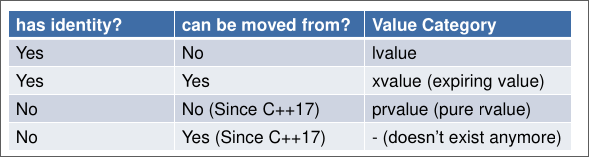
\includegraphics[scale=0.4]{2023_02_28_01_43_39.png}
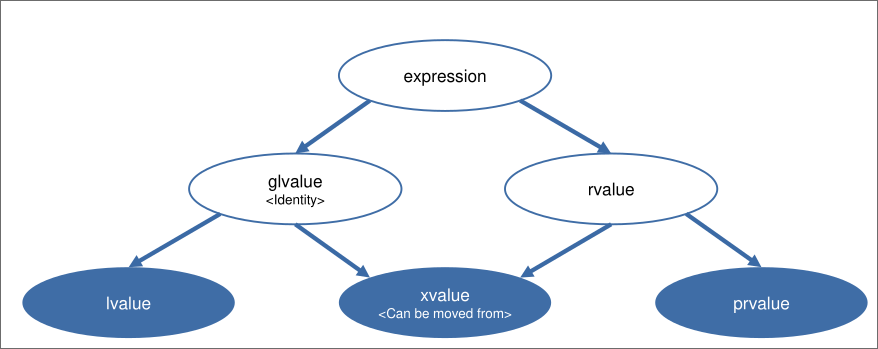
\includegraphics[scale=0.35]{2023_02_28_01_44_08.png}\newline
\begin{itemize}
\item \textcolor{purple}{lvalue}
  \begin{itemize}
  \item \textcolor{black}{address can be taken}
  \item \textcolor{black}{Can be on the left-hand side of an assignment if modifiable}
  \item \textcolor{black}{Can be used to initialize lvalue references}
  \item \textcolor{black}{Examples: variables, function calls that return reference, increment and decrement operators, array index access if array is lvalue}
  \item all string literals
  \end{itemize} 
\item \textcolor{purple}{prvalue}
  \begin{itemize}
  \item \textcolor{black}{address can't be taken -> doesn't exist}
  \item \textcolor{black}{cannot be on the left hand side of assignment}
  \item \textcolor{black}{temporary "materialization" to xvalue}
  \item \textcolor{black}{Examples: literals, false, nullptr, function call with non reference return type, postincrement and postdecrement!! }
  \end{itemize} 
\item \textcolor{purple}{xvalue}
  \begin{itemize}
  \item \textcolor{black}{address cannot be taken}
  \item \textcolor{black}{Cannot be used as left-hand operator of built-in assignment}
  \item \textcolor{black}{Conversion from prvalue through temporary materialization}
  \item \textcolor{black}{Examples: function calls with rvalue reference return type -> std::move, access of non-references members of an rvalue object, arra index access when array is rvalue}
  \end{itemize} 
\end{itemize}

\subsubsection{Temporary Materialization}
Getting from something imaginary to something you can point to....\newline
When this happens:\newline
\begin{itemize}
\item \textcolor{purple}{binding a reference to a prvalue}
\item \textcolor{purple}{when accessing a member of prvalue}
\item \textcolor{purple}{when accessing an element of a prvalue array}
\item \textcolor{purple}{when converting a prvalue array to a pointer}
\item \textcolor{purple}{when initializing an std::initializer\_list<T> from a braced-init-list}
\item \textcolor{red}{Type needs to be complete and needs to have a destructor}
\end{itemize} 
\begin{lstlisting}
struct Ghost {
  auto haunt() const -> void {
    std::cout << "booooo!\n";
  }
  //~Ghost() = delete;
};
auto evoke() -> Ghost {
  return Ghost{};
}
auto main() -> int {
  Ghost&& sam = evoke(); // bind reference to a prvalue
  Ghost{}.haunt(); // access member of prvalue
}
\end{lstlisting}

\subsection{l and rvalue references}
\begin{itemize}
\item \textcolor{purple}{lvalue reference} \textcolor{red}{made only of lvalues!!}
  \begin{itemize}
    \item type: T\&
  \item \textcolor{black}{alias for a variable}
  \item \textcolor{black}{can be used as function member type, local member/variable, return type}
  \item \textcolor{black}{be aware of dangling references when returning!}
  \end{itemize} 
\item \textcolor{purple}{rvalue reference} \textcolor{red}{made of rvalues, prvalues or xvalues!}
  \begin{itemize}
    \item \textcolor{black}{Type: T\&\&}
  \item \textcolor{black}{when assigned to a name (for example inside of a function), then it is actually an lvalue!!}
  \item \textcolor{black}{Argument is either a literal or a temporary object}\newline 
    \begin{lstlisting}
    std::string createGlass() -> std::string;
void fancyNameForFunction() { 
  std::string mug{"cup of coffee"};
  std::string&& glass_ref = createGlass(); //life-extension of temporary
  std::string&& mug_ref = std::move(mug); //explicit conversion lvalue to rvalue
  int&&
  i_ref = 5;
  //binding rvalue reference to prvalue
}
    \end{lstlisting}
  \end{itemize} 
\end{itemize} 

\subsection{Binds}
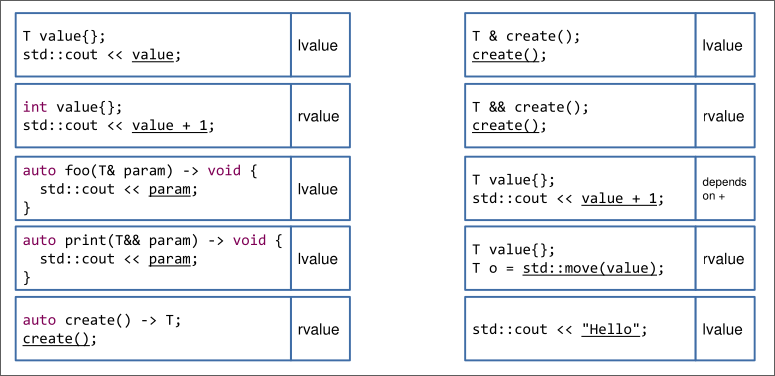
\includegraphics[scale=0.3]{2023_02_28_02_08_52.png}
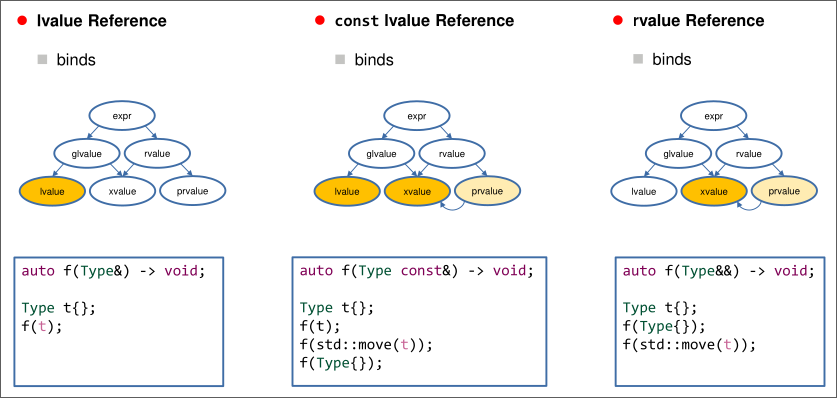
\includegraphics[scale=0.35]{2023_02_28_02_09_12.png}\newline
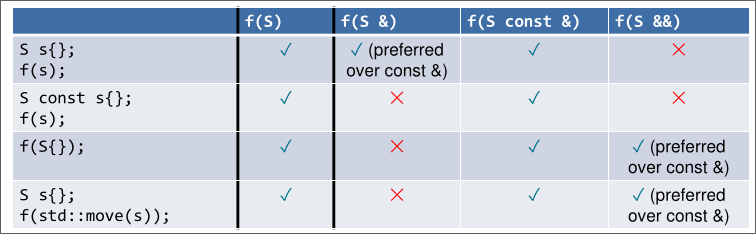
\includegraphics[scale=0.35]{2023_02_28_02_10_51.png}
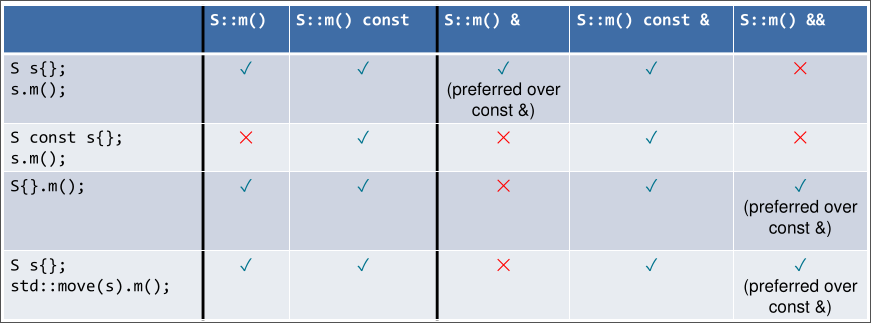
\includegraphics[scale=0.3]{2023_02_28_02_11_11.png}

\subsection{Destructor}
\textcolor{purple}{Whenever you need to write an explicit destructor, please make sure that you will not throw exeptions here. This can cause memory to not be freed, which.... well you guess what heppens}
\textcolor{teal}{In general you should make sure that \emph{ANY form of memory management doesn't throw exceptions!!!}}

\subsection{Default Constructors and user defined Constructors}
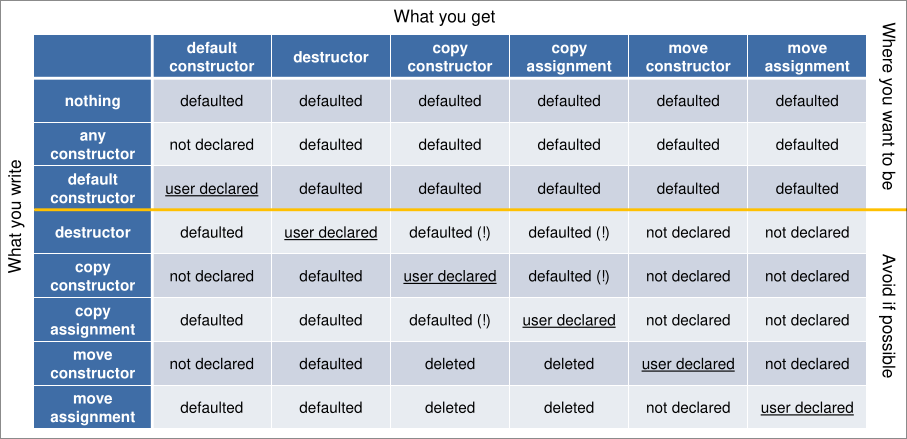
\includegraphics[scale=0.4]{2023_02_28_02_42_31.png}\newline
\textcolor{teal}{The ! means that it is a standard library bug, don't use those defaulted ones!!!}\newline
\textcolor{red}{Note that deleting a constructor will be the same as "user declared"!!}

\subsectin{The problem with func(T const\&)}
\textcolor{purple}{When working with const T references, this implies that we can either \emph{copy or move it}, this means we will not necessarily know what we get.}\newline
\textcolor{teal}{The only possible way without type deduction is an overload for both.}
\begin{lstlisting}
template <typename T>
  auto log_and_do(T const& param) -> void {
  //log
  do_something(param);
} // lvalue 
template <typename T>
  auto log_and_do(T&& param) -> void {
  //log
  do_something(std::move(param));
} // lvalue and rvalue!!
\end{lstlisting}
\textcolor{red}{Note, with more parameters, you would need x amount of overloads for each combination of parameters!!}

\section{Type Deduction}

\subsection{Forwarding Reference}
\textcolor{purple}{A T\&\& is not always an rvalue! In some cases, it is a forwarding reference, which can be either an lvalue or an rvalue!!}\newline
\begin{lstlisting}
template <typename T>
auto f(T && param) -> void;

// lvalue
int x = 23;
f(x);
// auto f(int & param) -> void; (inferred)

// rvalue
f(23);
// auto f(int && param) -> void; (inferred)
\end{lstlisting}

\subsection{Rules for Type Deduction}
\begin{lstlisting}
// base function
template <typename T>
auto f(T param) -> void;

// type usages with function instances and deduced T
int          x = 23; // f(x) = f(int param) -> T = int
int const   cx = x; // f(cx) = f(int param) -> T = int
int const& crx = x; // f(crx) = f(int param) -> T = int
char const * const ptr = /* something */; // f(ptr) = f(char const * param) -> T = char const*;
// -- ignore outermost const
// -- ignore reference types
// -- take base type

// base function 2 
template <typename T>
auto f(T & param) -> void;

// type usages with function instances and deduced T
int          x = 23;  // f(x) = f(int& param) -> T = int
int const   cx = x;   // f(cx) = f(int const& param) -> T =int const
int const& crx = x;   // f(crx) = f(int const& param) -> T = int const
// -- ignore reference type

// base function 3
template <typename T>
auto f(T const& param) -> void;

// type usages with function instances and deduced T
int          x = 23; // f(x) = f(int const& param) -> T = int
int const   cx = x;  // f(cx) = f(int const& param) -> T = int
int const& crx = x;  // f(crx) = f(int const& param) -> T = int
// -- ignore reference types
// -- take base type

// base function 4
template <typename T>
auto f(T&& param) -> void;

// type usages with function instances and deduced T
int          x = 23; // f(x) = f(int& param) -> T = int&
int const   cx = x;  // f(cx) = f(int const& param) -> T = int const&
int const& crx = x;  // f(crx) = f(int const& param) -> T = int const&
//                   // f(27) = f(int&& param) -> T = int 
// -- if param is an lvalue, then they become lvalue references
// -- otherwise rvalue, default rules for references

\end{lstlisting}

\subsubsection{Deducing Initializer Lists}
\textcolor{purple}{With initializer lists, you can't directly deduce the type as it will think T is the entire list, which is nonsense!}
\begin{lstlisting}
template <typename T>
auto f(T param) -> void;
f({23}); //error

template <typename T>
auto f(std::initializer_list<T> param) -> void;
f({23}); //T = int
//ParamType = std::initializer_list<int>
\end{lstlisting}

\subsubsection{Deducing auto types}
\begin{lstlisting}
autox = 23;         //auto is a value type
auto const cx = x;  //auto is a value type
auto& rx = x;       //auto is a reference type
auto&& uref1 = x;   //x is an lvalue, uref1 is int&
auto&& uref2 = cx;  //cx is an lvalue, uref2 is int const&
auto&& uref3 = 23;  //23 is an rvalue, uref3 is int&&

// special cases
auto init_list1 = {23};  //std::initializer_list<int>
auto init_list2{23};     //int, was std::initializer_list<int>
auto init_list3{23, 23}; //Error, requires one single argument
\end{lstlisting}
\textcolor{purple}{Note that auto type deduction works with parameters and return types, with the special cases like initializer list still applying!!}

\subsubsection{Type Deduction with Decltype}
\begin{lstlisting}
int           x       = 23;
int const     cx      = x;
decltype(cx)  cx_too  = cx; //type of cx_too is int const
int&          rx      = x;
decltype(rx)  rx_too  = rx; //type of rx_too is int&

// these two are the only surprises! auto only gives the base type without reference, while the other gives the full reference type
auto just_x = rx; //type of just_x is int
decltype(auto) more_rx = rx; //type of more_rx is int&
\end{lstlisting}
\textcolor{orange}{decltype(auto) etc can also be used for returning something specific:} 
\begin{lstlisting}
// auto decltype
template <typename Container, typename Index>
decltype(auto) access(Container & c, Index i) {
  return c[i];
}

// specific decltype
template <typename Container, typename Index>
auto access(Container & c, Index i) -> decltype(c[i]) {
  return c[i];
}
\end{lstlisting}
\textcolor{red}{Note we can only declare decltype(c[i]) as a trailing type! The reason for this is that c and i are only known AFTER the parameters!}

\subsubsection{Returns with decltype}
\begin{lstlisting}
decltype(auto) funcName() {
  int local = 42;
  return local; // decltype(local) => int
} // lvalue -> T
decltype(auto) funcNameRef() {
  int local = 42;
  int & lref = local;
  return lref; // int & -> bad (dangling)
} // lvalue reference -> T&
decltype(auto) funcXvalue() {
  int local = 42;
  return std::move(local); // int && -> bad (dangling)
} // rvalue reference -> T&&
decltype(auto) funcLvalue() {
  int local = 42;
  return (local); // int & -> bad (dangling)
} // lvalue reference -> T&
decltype(auto) funcPrvalue() {
  return 5; // int
} // prvalue -> T
\end{lstlisting}

\subsection{Checking for r and l-values}
\textcolor{purple}{We learned that we can solve the issue of multiple overloads with T\&\&, but what if we want to differentiate after the fact? std::forward!}
\begin{lstlisting}
template <typename T>
auto log_and_do(T&& param) -> void {
  //log
  do_something(std::forward<T>(param));
}

// example for implementation
template <typename T>
  decltype(auto) forward(std::remove_reference_t<T>& param) {
  return static_cast<T&&>(param);
}
// explanation
// this will check if we have an lvalue or not by trying to cast to an rvalue reference
// if & and && are casted, it will always result in &
// this means only an rvalue will result in an rvalue being returned, everything else will result in lvalue being returned
// this is called reference collapsing!
// example -> when T is int& the static cast will be int& && and hence collapsed to int&
// when T is int&& the static cast will be int&& && and hence collapsed to int&&
// when T is int, the static cast will be int&&, no collapse is needed here.
// note references are only checked for the type, the actual references are removed, as can be seen by the std::remove_reference_t
\end{lstlisting}
\textcolor{orange}{This means that forwards is essentially \emph{a conditional cast to an rvalue reference!}}\newline
Rules for reference collapsing:
\begin{itemize}
  \item \textcolor{purple}{\& and \& = \&}
  \item \textcolor{purple}{\&\& and \& = \&}
  \item \textcolor{purple}{\& and \&\& = \&}
  \item \textcolor{purple}{\&\& and \&\& = \&\&}
\end{itemize} 

\subsubsection{std::move vs std::forward}
\textcolor{purple}{While forward is the \emph{conditional cast}, std::move is the \emph{unconditional cast}! This means you will always receive an rvalue!}
\begin{lstlisting}
// std::forward
template <typename T>
  decltype(auto) forward(std::remove_reference_t<T>& param) {
  return static_cast<T&&>(param); 
} // will collapse dynamically
// std::move
template <typename T>
decltype(auto) move(T&& param) { // param is always T&& !!!
  return static_cast<std::remove_reference_t<T>&&>(param);
} // will always collapse to && and && meaning && is returned
\end{lstlisting}

\section{Lambdas}

\subsection{From lambda to actual code}
\begin{lstlisting}
// lambda
int i0 = 42;
auto missingMutable = [i0] {return i0++;};

// compiler code
struct CompilerKnows {
  auto operator()() const -> int {
    return i0++;
  }
  int i0;
};
\end{lstlisting}

\end{document}
